% Generated by reproduction/framework_experiments/build_manuscript_assets.py.
\subsection{Numerical evidence for the three questions}
\label{num:scope}
The experiments follow the three questions in the derivation: P1 checks
the matrix implementation and its stated geometric structure; P2 tests
residual compensation through the physical magnetic ports; P3 separates
convergence to the actual closed field from recovery of a nominal target.
All magnetic calculations use the newly sourced beam and endpoint-core
baseline. The synthetic matrix checks have their own declared,
dimensionless parameters. The reference-tracking extension is retained
in Supplementary Section~\ref{num:route-b}, with its distinct target and
assessment protocol.

Physical-input uncertainty, spatial and modal approximation, coefficient
identification, time integration and feedback error are different sources
of error. Mesh convergence does not measure a two-mode truncation error;
a small integral-fit residual does not bound an analytic norm; and a
small trajectory error does not establish an invariant-torus certificate.
The following tests assign a separate numerical question to each interface.

\subsection{P1: matrix implementation, order and structure}
\label{num:p1}
For $n=1,2,4$, set
\begin{equation}
 \begin{split}
 M&=\operatorname{diag}(1+j/5)_{j=0}^{n-1}
       +0.12\boldsymbol1\boldsymbol1^{\mathsf T},\\
 K&=\operatorname{diag}(1+j)_{j=0}^{n-1}
       +0.05\boldsymbol1\boldsymbol1^{\mathsf T},\qquad C=0.2M.
 \end{split}
 \label{num:matrix-data}
\end{equation}
These are artificial verification matrices, not catheter material
parameters. Each dimension uses a fixed initial state, $T=4$, and steps
$0.08,0.04,0.02,0.01$. Independent matrix exponentials are evaluated at
every point of the finest common time grid. The error is the maximum
Euclidean state error over all saved times, rather than only the endpoint.
For $n=2,4$, $M$ and $K$ do not commute.

The full ordinary-midpoint solve and the correctly ordered eliminated
update agree over their entire trajectories to at most
$5.3959\times10^{-15}$. A second algebraic family uses
$C_g=0.2M+0.03vv^{\mathsf T}/(v^{\mathsf T}v)$, $v=(1,\ldots,n)^{\mathsf T}$.
It checks the order of $C_gM^{-1}$ as well: $C_g$ is nonproportional for
$n=2,4$, while $n=1$ is necessarily a scalar comparison. Its maximum
trajectory discrepancy is $4.6926\times10^{-15}$. No common exponential
weighted-structure claim is assigned to that additional family.

\begin{table*}[t]
\centering
\caption{P1 matrix verification. Orders use full-grid maximum errors at the final step halving. The conservative columns use the quadratic target with stiffness $K+K_s$, $K_s=0.05\operatorname{diag}(1,\ldots,n)$.}
\label{num:matrix-benchmark}
\small
\begin{tabular}{rccccc}
\toprule
$n$ & Max. elimination difference & Ordinary midpoint & Weighted midpoint & Conservative midpoint & Conservative Central4\\
\midrule
1 & $1.144\times10^{-15}$ & $1.999964$ & $1.999942$ & $1.999944$ & $3.999945$ \\
2 & $4.767\times10^{-15}$ & $1.999935$ & $1.999876$ & $1.999890$ & $3.999813$ \\
4 & $5.396\times10^{-15}$ & $1.999869$ & $1.999821$ & $1.999823$ & $3.999864$ \\
\bottomrule
\end{tabular}
\end{table*}

The ordinary damped midpoint and the weighted Birkhoff midpoint both
converge at order two, but their geometric diagnostics differ. At
$n=2$, $\Delta=0.08$, the ordinary map has exponential-weighted defect
$3.9280\times10^{-5}$, whereas the weighted map has defect
$1.1631\times10^{-16}$. Here the defect is
$\|D\Psi^{\mathsf T}JD\Psi-e^{-0.2\Delta}J\|_2$.
For the conservative quadratic target, midpoint and Central4 have
standard symplectic defects at rounding scale and orders two and four,
respectively. The shaping input is exactly specified; no fourth-order
conclusion is assigned to an arbitrary damped feedback update.

The same distinction is checked on the full nonlinear magnetic potential
using the new physical coordinates. For the uncompensated synthetic
plant, ordinary and weighted midpoint have final observed orders
$1.999452$ and $1.999400$ over $0\leq\tau\leq4$.
At $\Delta=0.04$, the ordinary exponential-weighted defect is
$2.8763\times10^{-5}$; the maximum weighted-map defect over all
tested steps is $4.4412\times10^{-16}$. The corresponding known-error
closed-field comparison gives the same structural distinction.
These tests evaluate the implicit ideal tangent at solved numerical
points. They neither establish exact symplecticity of floating-point
Newton code nor give a learning controller access to unknown errors.

\begin{figure*}[t]
\centering
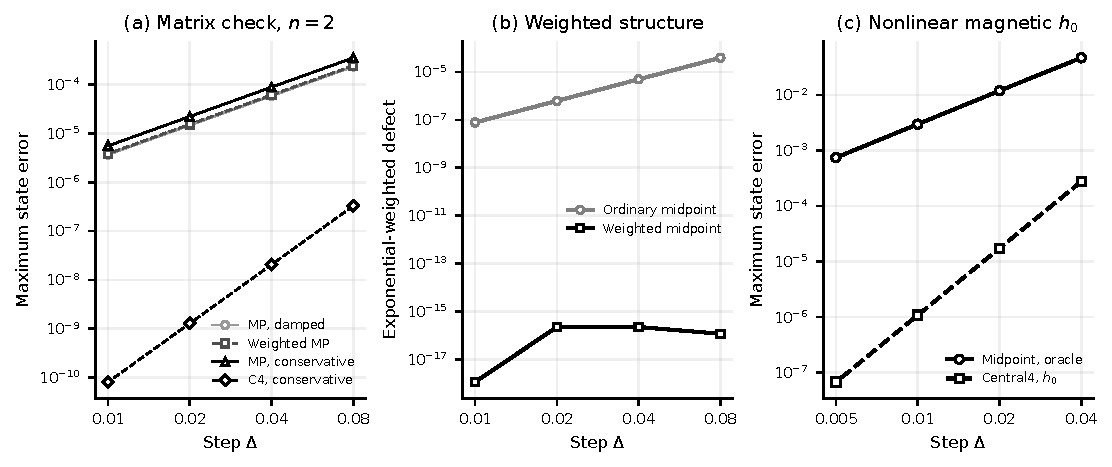
\includegraphics[width=\textwidth]{figures/framework_matrix_checks.pdf}
\caption{P1 checks of the implemented maps. (a) Full-grid matrix errors for $n=2$ against independent matrix exponentials; the damped and conservative groups have their own declared exact targets. (b) Exponential-weighted defects for ordinary and weighted damped midpoint. (c) Midpoint and Central4 on the same nonlinear conservative magnetic $h_0$; these curves compare discretizations of one Hamiltonian. All coordinates, matrices, initial states and reference settings are in the JSON records.}
\label{num:matrix-structure}
\end{figure*}

\subsection{Common physical baseline and modal coordinates}
\label{num:fe}
The benchmark uses the paired material references $E\simeq2.1$ MPa and
$\rho\simeq1028$ kg/m$^3$, with the preparation stated by
\citet{cho2021pdms}. The free length $80$ mm and radius $0.6$ mm are
research design inputs. The nominal $0.250$ mm magnetic cube uses
$B_r=1.425$ T and density $7500$ kg/m$^3$, with their manufacturer-grade
and nominal-selection status retained \citep{smN50,kjMoment}.
Its translational mass and rotary inertia enter the FE mass matrix before
reduction. The consistent $16/32/64$-element frequencies are compared
with independent continuum boundary roots. The largest relative error
among the first four modes is $9.59029\times10^{-6}$ at $32$ elements and
$6.02081\times10^{-7}$ at $64$ elements (Table~\ref{sx:fe-table}).

The adopted $32$-element coordinates are
\begin{align}
 \omega_0=\omega_1&=7.84000916\ \mathrm{rad/s},\notag\\
 \omega_2&=47.39957662\ \mathrm{rad/s},\qquad
 \nu_2=6.04585730,\notag\\
 d&=\bigl(0.30722439,\,0.45042632\bigr)^{\mathsf T},\notag\\
 \ell&=\bigl(0.0189673443,\,0.0077534761\bigr)^{\mathsf T}\ \mathrm m.
 \label{num:scales}
\end{align}
The generator, controls and physical readouts use these same maps.
The declared baseline $C=\alpha M_{\mathrm{total}}$ has
$\zeta_1^{\mathrm d}=0.025$, $\alpha=0.3920004581$ s$^{-1}$ and
$\gamma=0.05$, giving $\zeta_2^{\mathrm d}=0.0041350629$.
These damping ratios are design choices, not measured losses of the
declared beam. Material, inertia and remanence sensitivity points are
reported separately in Table~\ref{sx:sensitivity-table}; they are not
confidence intervals or high-mode control validation.

\subsection{P2: learned residual compensation through the magnetic ports}
\label{num:p2}
\label{num:route-a}
The controlled synthetic departure from $h_0$ is a single potential
feature. Define
\begin{equation}
 \begin{split}
 \phi(X)&=\nabla_X g(d^{\mathsf T}X)\\
        &=d[\sin(d^{\mathsf T}X)-d^{\mathsf T}X],
 \end{split}
 \label{num:feature-gradient}
\end{equation}
and
\begin{equation}
 \begin{split}
 R_*(X)&=\beta_*g(d^{\mathsf T}X),\qquad \beta_*=0.2,\\
 \widehat R(X)&=\widehat\beta g(d^{\mathsf T}X).
 \end{split}
 \label{num:feature}
\end{equation}
The coefficient $0.2$ is a declared stress-test setting, not an identified
material discrepancy. Together with the drag coefficient, this gives a
two-scalar fit. Its recovery does not measure full CHNN optimization or
generalization across richer residual families.

\label{num:identification}
Four training trajectories and two disjoint validation trajectories each
last $\tau=4$. Noiseless states are observed every $0.002$, and Simpson
windows of length $0.04$ produce $400$ training vector increments,
or $800$ scalar rows. For $W=[\tau_a,\tau_b]$ the balance is
\begin{equation}
 \begin{split}
 b_W&=Y_b-Y_a+\int_W\{\mathsf NX+\phi(X)\}\,\mathrm d\tau,\\
 A_W&=\left[-\int_W\phi(X)\,\mathrm d\tau,
                 -\int_WY\,\mathrm d\tau\right],\\
 A_W\binom{\beta}{\gamma}&\simeq b_W.
 \end{split}
 \label{num:regression}
\end{equation}
Column-scaled, unconstrained least squares gives
\begin{equation}
 \widehat\beta=0.200003368491,\qquad
 \widehat\gamma=0.04999999998680.
 \label{num:fitted-values}
\end{equation}
Training and held-out increment RMS residuals are $1.0123\times10^{-12}$ and
$9.2492\times10^{-13}$. The raw and scaled design condition numbers are
$10418.25$ and $1.04537179$. The normalized Gram matrix has
$\lambda_{\min}(G)=5.15486\times10^{-14}$, so weak feature excitation still
matters despite a well-conditioned scaled solve. The truth-dependent
coefficient error $3.36849\times10^{-6}$ is a synthetic diagnostic; an
independently justified integration/observation defect bound remains
necessary for the analytic estimates of Section~\ref{sec:kam}.

All four restoration groups start at
$(0.09,0.08,0.015,-0.01)$ and run to $\tau=20$ ($2.551017$ s),
using midpoint step $0.001$. Every nonzero command is converted to
physical magnetic force/torque and field/gradient, reconstructed and
substituted into the plant during integration. Only the declared oracle
uses true coefficients. Each group is compared with an independently
integrated $h_0$ trajectory from the same initial state.

\begin{table*}[t]
\centering
\caption{P2 restoration through the same physical port map. State and tip RMS use an independent $h_0$ RK4 reference; energy change is the dimensionless nominal quantity $\max_k|h_0(x_k)-h_0(x_0)|$.}
\label{num:a-table}
\begin{tabular}{lccc}
\toprule
Control & State RMS & Tip RMS ($\mu$m) & Maximum nominal energy change\\
\midrule
Passive & $2.92453\times10^{-2}$ & $322.376137$ & $1.50142\times10^{-2}$ \\
Damping compensation & $2.43437\times10^{-5}$ & $0.143531$ & $1.37056\times10^{-7}$ \\
Learned restoration & $1.71438\times10^{-5}$ & $0.094120$ & $5.64520\times10^{-12}$ \\
Oracle restoration & $1.71439\times10^{-5}$ & $0.094120$ & $3.24493\times10^{-12}$ \\
\bottomrule
\end{tabular}
\end{table*}

The fitted restoration reduces the state RMS to $1.71438\times10^{-5}$
and the tip RMS to $0.094120\,\mu$m in this ideal two-mode test.
Its sampled continuous-field mismatch has RMS $2.5942\times10^{-11}$, yet its
trajectory error remains close to the oracle's $1.71439\times10^{-5}$:
both include the same midpoint phase error. A slightly smaller learned
error is compatible with cancellation of two small errors and is not
evidence of outperforming true parameter knowledge. This is restoration
from a shared initial state, not attraction from a tracking offset.

\subsection{P3: convergence to the actual controlled dynamics}
\label{num:p3}
\label{num:integration}
The principal nonlinear oracle midpoint test is retained. Step halvings
$0.04,0.02,0.01,0.005$ give final order $1.999331$ against an
independent RK4 reference, whose step-refinement difference is
$6.3600\times10^{-12}$. A new Central4 test uses the same full-cosine conservative
$h_0$, with all derivatives in Supplementary equation~\eqref{ss:central4-magnetic-jacobian}; it does not append a control
kick after an unrelated map. Its final order is $3.999503$.
The independent DOP853 reference-refinement difference is
$1.1642\times10^{-11}$, below the smallest reported Central4 error.
The analytic increment Jacobian agrees with complex-step differentiation
to $2.7756\times10^{-17}$ at the specified check states.

\begin{table*}[t]
\centering
\caption{Nonlinear conservative $h_0$ integration to $\tau=20$. Errors are maxima over saved times against independent references. Midpoint is the existing perfect-compensation test; Central4 is the new conservative method check.}
\label{num:nonlinear-order}
\begin{tabular}{rcccc}
\toprule
$\Delta$ & Midpoint error & Midpoint order & Central4 error & Central4 order\\
\midrule
$0.04$ & $4.64310\times10^{-2}$ & --- & $2.75432\times10^{-4}$ & --- \\
$0.02$ & $1.18409\times10^{-2}$ & $1.971306$ & $1.73275\times10^{-5}$ & $3.990559$ \\
$0.01$ & $2.96760\times10^{-3}$ & $1.996414$ & $1.08474\times10^{-6}$ & $3.997648$ \\
$0.005$ & $7.42245\times10^{-4}$ & $1.999331$ & $6.78193\times10^{-8}$ & $3.999503$ \\
\bottomrule
\end{tabular}
\end{table*}

To distinguish convergence from model recovery, a separate experiment
freezes the deliberately nonzero identification errors
$\delta\beta=0.02$, $\delta\gamma=0.01$. Thus the controller uses
$\widehat\beta=0.18$, $\widehat\gamma=0.04$ on the same declared plant.
These are manufactured test errors, not outputs of the preceding fit or
measured uncertainty. The actual field is
\begin{equation}
 \begin{split}
 X'&=\mathsf NY,\\
 Y'&=-\mathsf NX-(1+0.02)\phi(X)-0.01Y.
 \end{split}
 \label{num:fixed-error-field}
\end{equation}
The midpoint loop still uses the physical command reconstruction. An
independent DOP853 implementation integrates the explicitly reduced field
above; their sampled field difference is at most $1.1189\times10^{-16}$.
The control coefficients stay frozen for every step size.

\begin{table*}[t]
\centering
\caption{P3 with fixed nonzero identification error. The first error is relative to the same actual continuous closed field; the final column is relative to nominal $h_0$. Both are full-grid maximum Euclidean errors.}
\label{num:closed-convergence}
\begin{tabular}{rccc}
\toprule
$\Delta$ & Error to actual closed field & Observed order & Error to nominal $h_0$\\
\midrule
$0.04$ & $4.20319\times10^{-2}$ & --- & $4.56736\times10^{-2}$ \\
$0.02$ & $1.07152\times10^{-2}$ & $1.971829$ & $1.60584\times10^{-2}$ \\
$0.01$ & $2.68521\times10^{-3}$ & $1.996545$ & $1.17602\times10^{-2}$ \\
$0.005$ & $6.71600\times10^{-4}$ & $1.999364$ & $1.14312\times10^{-2}$ \\
$0.0025$ & $1.67917\times10^{-4}$ & $1.999855$ & $1.14090\times10^{-2}$ \\
\bottomrule
\end{tabular}
\end{table*}

The actual-field error reaches $1.67917\times10^{-4}$ with final order
$1.999855$, while the nominal-target error approaches
$1.14090\times10^{-2}$. Independently integrating the two continuous
models gives a maximum difference $1.14070\times10^{-2}$ on the
finest common grid. Step reduction therefore resolves the actual closed
dynamics but does not eliminate the prescribed modeling error.
The independent reference-refinement difference is $1.0636\times10^{-11}$.
This directly illustrates the scope of the convergence estimate
\eqref{ctrl:global-error}.

\label{num:defect-budget}
A separate one-degree-of-freedom harmonic diagnostic tests its algebraic
residual term. In two-dimensional phase space, we deliberately solve
the perturbed midpoint increment equation with
$r_k=0.01\Delta^q(1,0)^{\mathsf T}$, $q=1,2,3$, over $T=4$.
Every actual original-equation residual is stored. This is a manufactured
algebraic defect, not a measured Newton stopping error or a catheter
experiment. Relative to the unperturbed midpoint trajectory, the added
error has final orders $0.000000,\,1.000000,\,2.000000$; its ratio to
$\eta_\Delta/\Delta$ is approximately $1.999999$.
The total error against the continuous oscillator has final orders
$0.000566,\,1.018776,\,1.999969$, respectively. In particular $q=3$ retains
second order; $q=1$ leaves a nonvanishing error. The test checks the
budget scaling, not a sharp universal value of the theorem's constant.

\begin{figure*}[t]
\centering
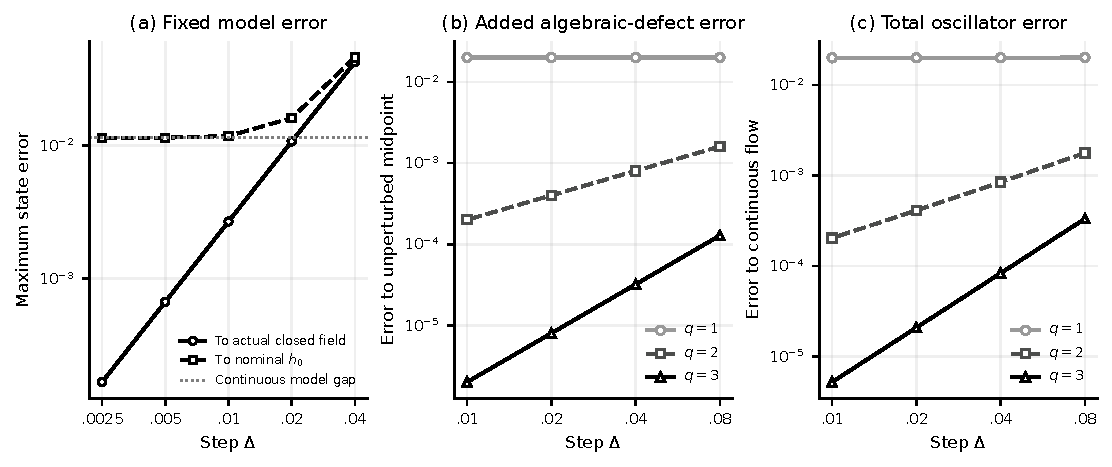
\includegraphics[width=\textwidth]{figures/framework_closed_loop_checks.pdf}
\caption{P3 separates numerical and model errors. (a) With fixed $\delta\beta=0.02$, $\delta\gamma=0.01$, midpoint converges to the actual closed field while its error to $h_0$ approaches the continuous model gap. (b) Added error caused by the manufactured increment defects, measured against unperturbed midpoint. (c) Total error against the independent continuous oscillator; only this diagnostic uses the separate one-degree-of-freedom test model.}
\label{num:closed-results}
\end{figure*}

\subsection{Damping scenarios, sampled domains and remaining boundaries}
\label{num:damping}
The additional ratios $\zeta_1^{\mathrm d}\in\{0,0.01,0.025,0.05,0.1\}$
each receive newly generated training/validation trajectories and a new
fit. Restoration uses $\tau\in[0,10]$, midpoint step $0.002$ and an
independent RK4 reference. Table~\ref{sx:framework-damping-a} reports
passive, learned and oracle groups. This is an in-family sensitivity
study, not one frozen controller resisting unknown damping changes.
The implemented estimator is explicitly unconstrained; it does not
silently implement a nonnegative constrained fit. At zero true damping
it returns $\widehat\gamma=-1.4038\times10^{-12}$, a numerical value that
is not interpreted as negative material loss. Material loss depends on
preparation and frequency and cannot identify these modal ratios without
an additional model or device measurement \citep{fischer2017adhesion}.

\label{num:ports}
The magnetic port matrix has column-normalized condition number
$3.8185963$; its differently dimensioned columns preclude interpreting
a raw condition number as a unit-independent measure.
The principal learned-restoration demands are
$\max|B_y|=0.544490$ mT and
$\max\|\nabla B\|_2=0.01603429$ T/m. Including the longitudinal bias,
the maximum local field is $30.004941$ mT. Published magnetic
systems offer a field-scale comparison \citep{lussi2021cvs}, not a
simultaneous field/gradient feasibility or bandwidth certificate for
these commands. The sampled endpoint angle and whole-beam slope remain
within the declared small-slope diagnostic domain; no continuous-time
or spatial extrema are certified.

No saturation or input-work governor is executed. For a net $4$ mm
clearance, $E_c=10.019717$ nJ and $0.95E_c=9.518731$ nJ,
whereas the principal initial nominal energy is $12.656721$
nJ. The proposed sufficient energy-cap premise is therefore not met
at initialization. The framework tests establish matrix consistency,
specific orders, algebraic port realization and the stated convergence
distinctions. Full-network fitting, higher-mode forced trajectories,
COMSOL comparisons, long-time frequency studies and finite-domain KAM
certificates remain separate tasks. Supplementary
Section~\ref{sx:migration} preserves the status of those earlier results.
